%!TEX root = main.tex
\section{Deliverable 1}
\label{sec:deliverable-1}

\subsection{Math Equations}
For example, one can type the following equation:
\begin{equation}
\vt^W = \MR_r^W \vt^r = \left[\begin{array}{ccc}
1 & 0 & 0 \\
0 & 1 & 0 \\
0 & 0 & 1
\end{array} \right]
\left[\begin{array}{c}
1\\
1 \\
1
\end{array} \right]
= 
\left[\begin{array}{c}
1\\
1 \\
1
\end{array} \right].
\end{equation}

Later in the course, you may want to type an optimization problem:
\begin{eqnarray}
f^\star = \min_{\vxx \in \mathbb{R}^n} & f(\vxx), \label{eq:optimization}\\
\text{subject to}  & \vxx \in \calX,
\end{eqnarray}
and refer to this optimization as problem~\eqref{eq:optimization}. For mathematical symbols, it is suggested that you define shortcuts to commonly used symbols and formats.

\subsection{Lists}
You may also make your answers more organized by using \emph{bulleted list}:
\begin{itemize}
	\item Observation 1 ...
	\item Observation 2 ...
\end{itemize}
and \emph{numbered list}:
\begin{enumerate}
	\item Observation 1 ...
	\item Observation 2 ...
\end{enumerate}

\subsection{Citations}
You can make a citation to a paper by~\cite{horn87josa-registration}.

\subsection{Figures}
You can also include a plot in Fig.~\ref{fig:simplefig}.

%!TEX root = main.tex
\begin{figure}[h]
\begin{center}
	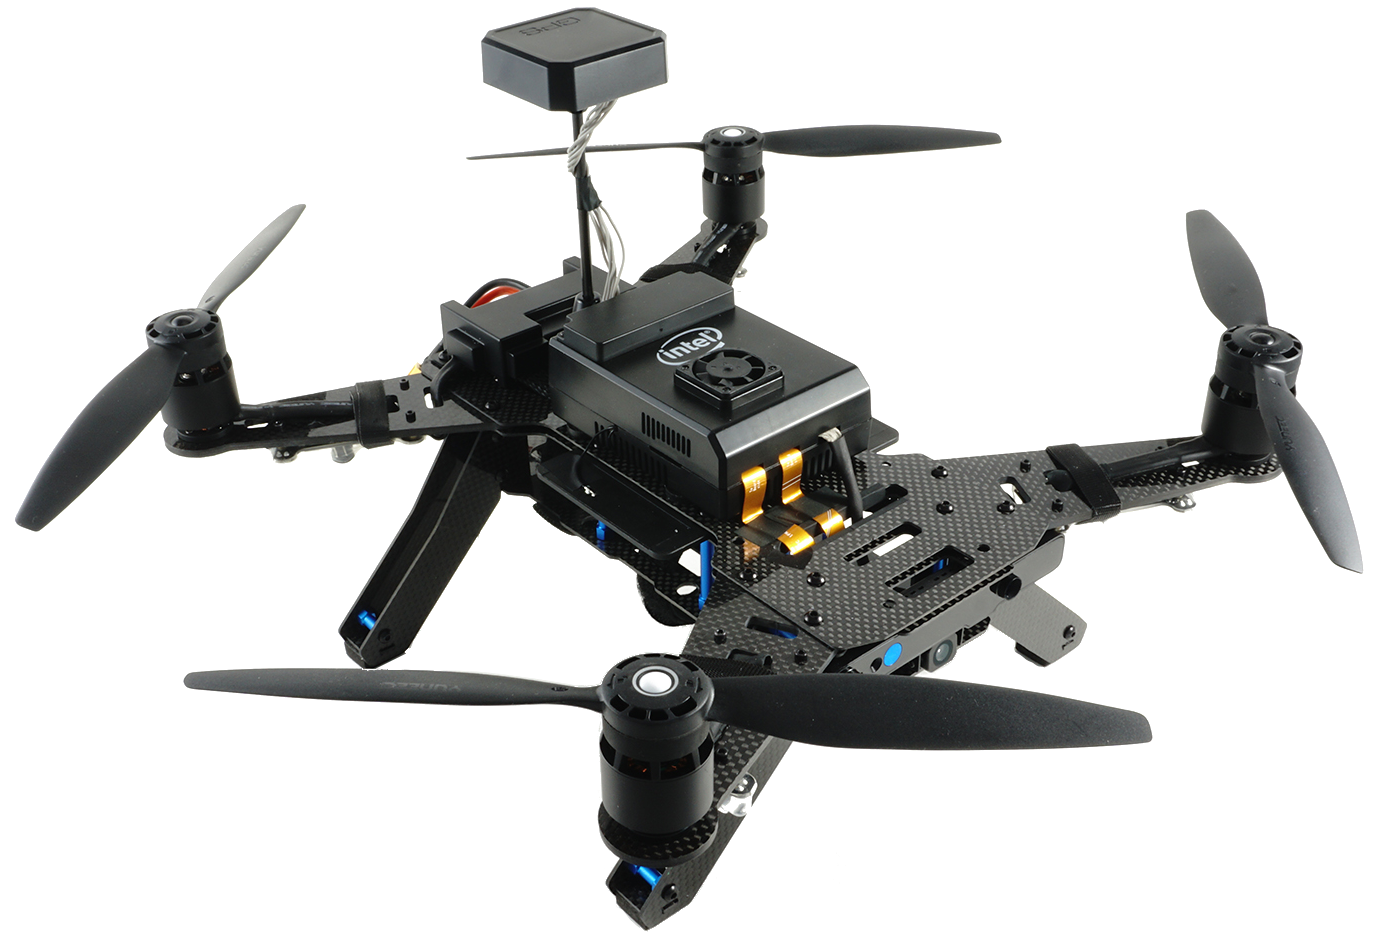
\includegraphics[width=0.5\columnwidth]{intel-aero-alpha.png} \\
	\caption{A drone. \label{fig:simplefig}}
\end{center}
\end{figure}